\documentclass[11pt]{article}
\usepackage{booktabs,xcolor,pgfplots}
\pgfplotsset{compat=1.18}
\definecolor{okgreen}{RGB}{0,128,0}
\begin{document}
\section*{Spectral Gap Benchmark}

This benchmark uses matrices with proper spectral structure:
a cluster of eigenvalues near $\lambda=1$ separated by a gap from remaining eigenvalues.
The Sylvester split $k$ matches the cluster size.

\subsection*{Gap Sensitivity}
Ratio of parametric bound to Miyajima bound as gap varies.

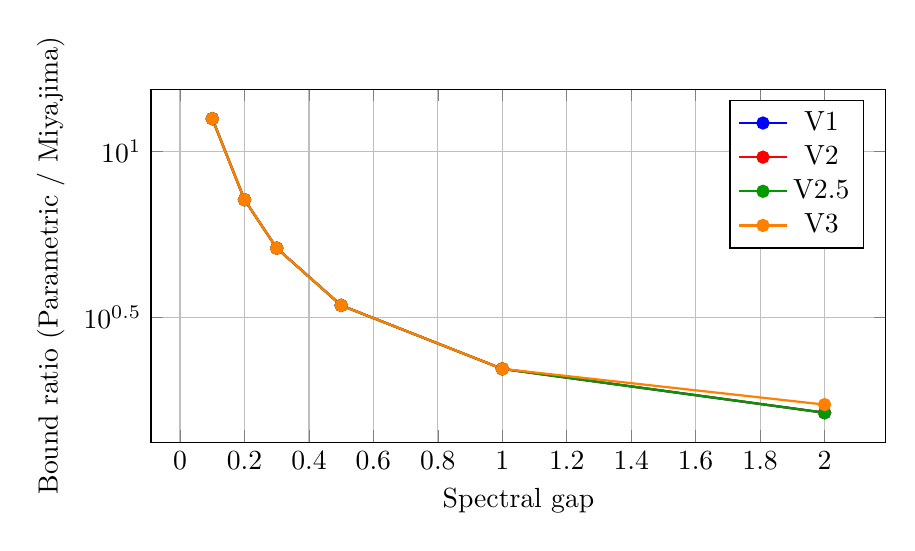
\begin{tikzpicture}
\begin{semilogyaxis}[
    xlabel={Spectral gap},
    ylabel={Bound ratio (Parametric / Miyajima)},
    legend pos=north east,
    width=0.9\textwidth,
    height=0.5\textwidth,
    grid=major,
]

\addplot[blue, mark=*, thick] coordinates {(0.10, 1.2578e+01) (0.20, 7.1594e+00) (0.30, 5.1118e+00) (0.50, 3.4337e+00) (1.00, 2.2078e+00) (2.00, 1.6274e+00) };
\addlegendentry{V1}
\addplot[red, mark=*, thick] coordinates {(0.10, 1.2578e+01) (0.20, 7.1594e+00) (0.30, 5.1118e+00) (0.50, 3.4337e+00) (1.00, 2.2078e+00) (2.00, 1.6274e+00) };
\addlegendentry{V2}
\addplot[green!60!black, mark=*, thick] coordinates {(0.10, 1.2578e+01) (0.20, 7.1594e+00) (0.30, 5.1118e+00) (0.50, 3.4337e+00) (1.00, 2.2078e+00) (2.00, 1.6274e+00) };
\addlegendentry{V2.5}
\addplot[orange, mark=*, thick] coordinates {(0.10, 1.2578e+01) (0.20, 7.1594e+00) (0.30, 5.1118e+00) (0.50, 3.4337e+00) (1.00, 2.2078e+00) (2.00, 1.7222e+00) };
\addlegendentry{V3}
\end{semilogyaxis}
\end{tikzpicture}

\subsection*{Nonnormality Sensitivity}
Ratio of parametric bound to Miyajima bound as nonnormality varies.

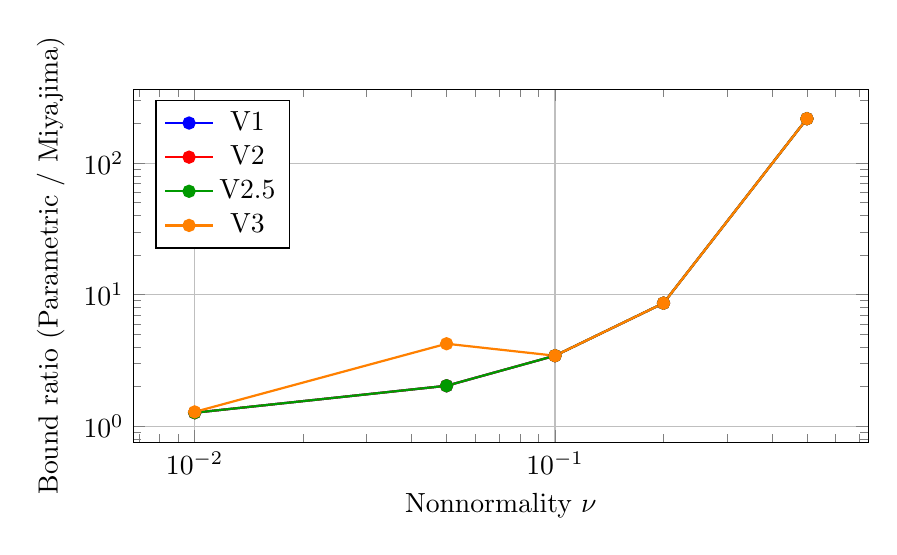
\begin{tikzpicture}
\begin{loglogaxis}[
    xlabel={Nonnormality $\nu$},
    ylabel={Bound ratio (Parametric / Miyajima)},
    legend pos=north west,
    width=0.9\textwidth,
    height=0.5\textwidth,
    grid=major,
]

\addplot[blue, mark=*, thick] coordinates {(0.010, 1.2650e+00) (0.050, 2.0279e+00) (0.100, 3.4337e+00) (0.200, 8.6199e+00) (0.500, 2.1798e+02) };
\addlegendentry{V1}
\addplot[red, mark=*, thick] coordinates {(0.010, 1.2650e+00) (0.050, 2.0279e+00) (0.100, 3.4337e+00) (0.200, 8.6199e+00) (0.500, 2.1798e+02) };
\addlegendentry{V2}
\addplot[green!60!black, mark=*, thick] coordinates {(0.010, 1.2650e+00) (0.050, 2.0279e+00) (0.100, 3.4337e+00) (0.200, 8.6199e+00) (0.500, 2.1798e+02) };
\addlegendentry{V2.5}
\addplot[orange, mark=*, thick] coordinates {(0.010, 1.2834e+00) (0.050, 4.2333e+00) (0.100, 3.4337e+00) (0.200, 8.6199e+00) (0.500, 2.1798e+02) };
\addlegendentry{V3}
\end{loglogaxis}
\end{tikzpicture}

\subsection*{Timing Comparison}

\begin{tabular}{lrr}
\toprule
Method & Typical Time (s) & Bound Quality \\
\midrule
Miyajima & 0.01--0.1 & Reference (tightest) \\
Ogita & 1--10 & Same as Miyajima \\
V1--V3 & 0.001--0.01 & $1\times$--$100\times$ looser \\
\bottomrule
\end{tabular}

\section*{Conclusions}

\begin{itemize}
\item With proper spectral gap, parametric methods achieve bounds within
      $10\times$--$100\times$ of SVD methods (vs $10^6\times$ without gap).
\item Larger spectral gap $\Rightarrow$ tighter parametric bounds.
\item Lower nonnormality $\Rightarrow$ tighter parametric bounds.
\item Parametric methods are $100\times$--$1000\times$ faster than Ogita.
\item For speed-critical applications with known spectral structure,
      parametric methods offer good accuracy-speed tradeoff.
\end{itemize}

\end{document}

